\chapter{Benutzeroberfläche}
\setcounter{counterKriterien}{0}


\gls{OQAT} stellt dem Nutzer eine intuitive graphische Oberfläche zur Verfügung.
Die Graphische Oberfläche setzt sich aus folgenden Bestandteilen zusammen:

\nItem{GUI} Hauptmenüleiste\\
Über das Hauptmenü sind nahezu alle Funktionen von \gls{OQAT} abrufbar. Das Hauptmenü ist das oberste
Element das auf den untenstehenden Abbildungen zu sehen ist.

\nItem{GUI} Toolbar\\
Über die Toolbar sind häufig benötigte Funktionen wie z.B. ">Neues Projekt erstellen"<, ">Projekt öffnen"< abrufbar. Die Toolbar ist das Element unterhalb der Hauptmenüleiste.

\nItem{GUI} Projektexplorer\\
Der Projektexplorer ist der Tabcontainer und auf der linken Seite der unten aufgeführten Screenshots zu sehen. Im Projektexplorer befindet sich der SmartTree und der Dateiexplorer.

\nItem{GUI} Filter und Metriken\\
Auf Filter und Metriken kann man über den rechten Tabcontainer zugreifen.

\nItem{GUI} Hauptvisualisierungsbereich\\
Im Hauptvisualisierungsbereich befindet sich der .YUV Player und außerdem werden hier die Ergebnisse einer
Analyse dargestellt.
\begin{figure}[p]
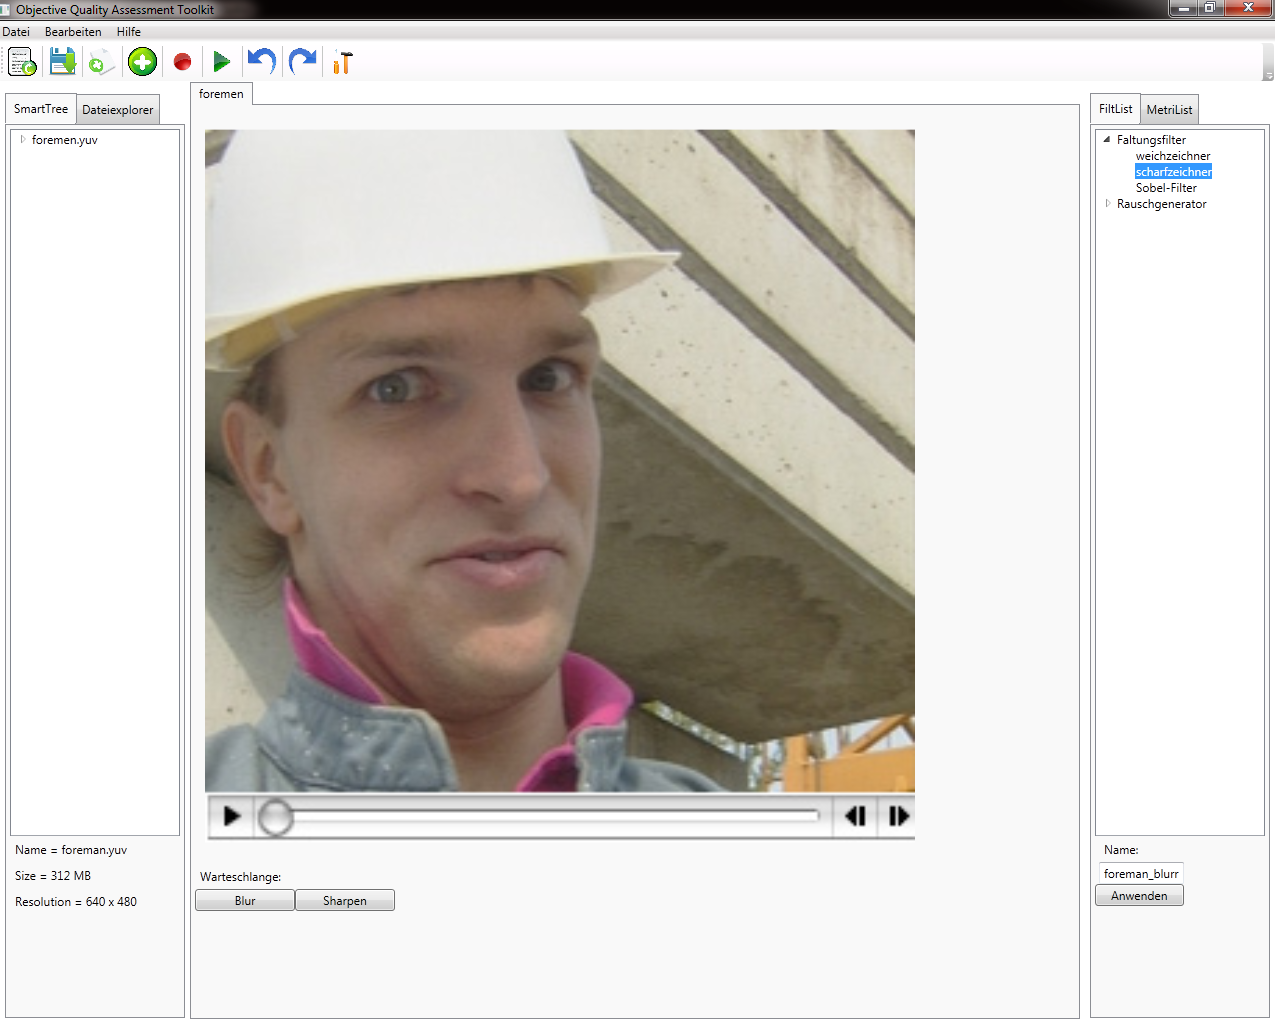
\includegraphics[scale=0.35]{bilder/screenFilter.png}
\caption{Auswahl mehrerer Filter und des Namens unter dem das so entstandene Video im
Projektordner gespeichert werden soll}
\label{screenFilter}
\end{figure}
\begin{figure}[p]
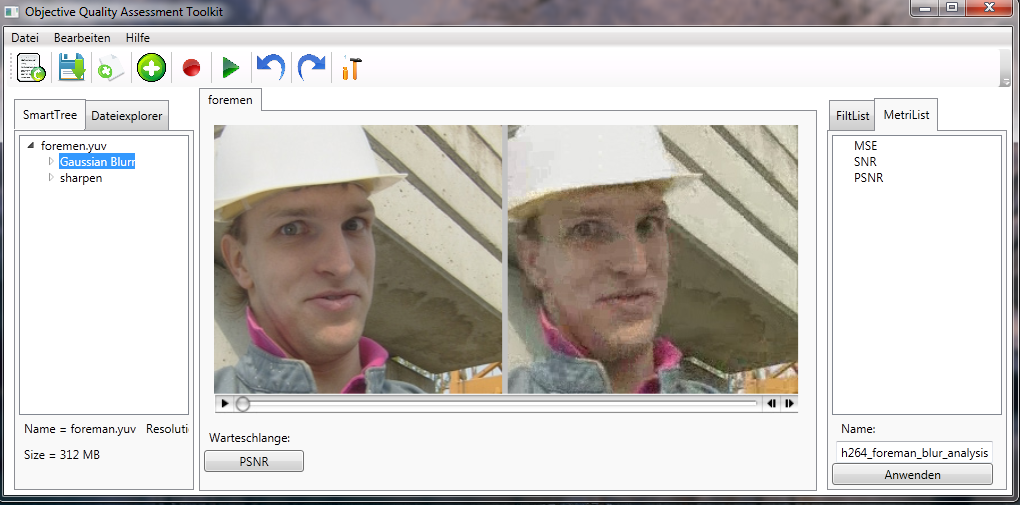
\includegraphics[scale=0.6]{bilder/screenAnalys.png}
\caption{Auswahl einer Analysemetrik und des Namens unter dem die Ergebnisdaten im 
Projektordner abgelegt werden sollen}
\label{screenAnalys}
\end{figure}
\begin{figure}[p]
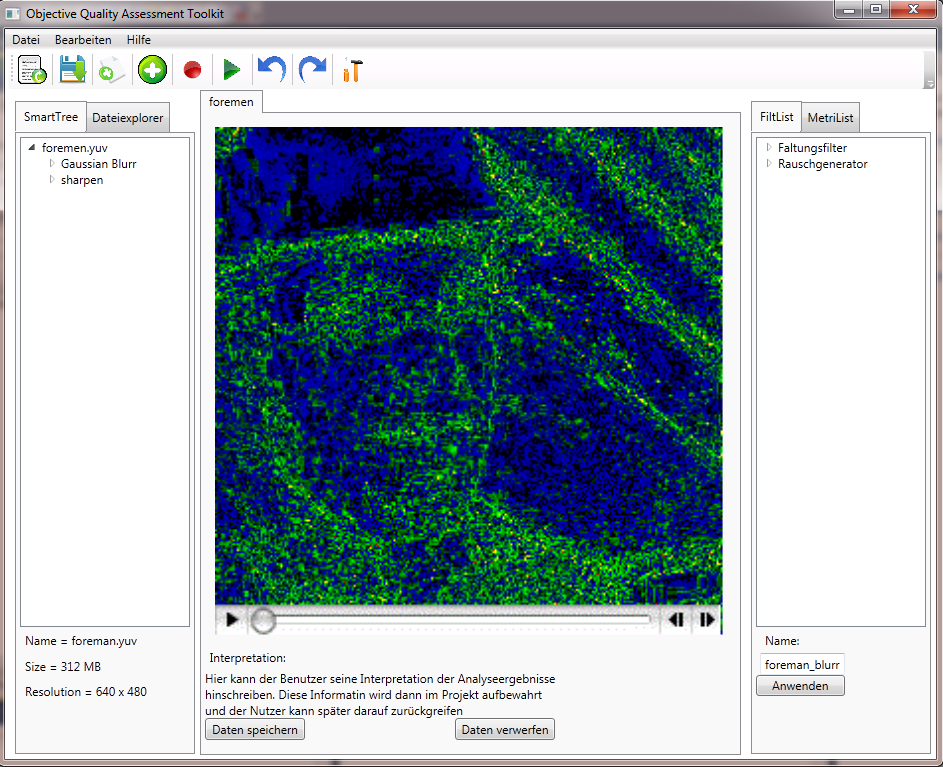
\includegraphics[scale=0.6]{bilder/screenResults.png}
\caption{Visuelle Darstellung der Ergebnisse nach einem Analysevorgang mit der \gls{psnr} Metrik}
\label{screenResults}
\end{figure}
